\setcounter{section}{6}
\section{Preparation Activity 7 - Context-Free Grammars (CFGs)}
{
\renewcommand{\thesubsubsection}{\thesubsection\alph{subsubsection}}
\subsection{Exercise 1}
\subsubsection{Item a}
\begin{definition}[CFG ambiguity]
A CFG is \textit{ambiguous} iff there exists a string $w$ that has at least two different syntax trees.
\end{definition}
This CFG is ambiguous, because the string $a+a \times a$ has two different syntax trees:
\begin{center}
\begin{minipage}{0.4\linewidth}
	\begin{center} 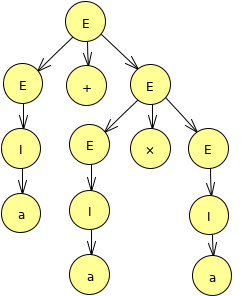
\includegraphics[scale=0.45]{PA07_1a_1} \end{center}
\end{minipage}
\begin{minipage}{0.4\linewidth}
	\begin{center} 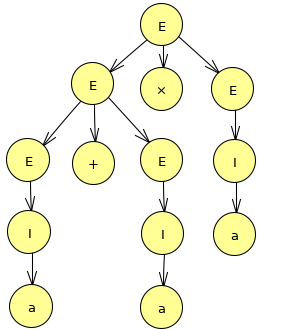
\includegraphics[scale=0.45]{PA07_1a_2} \end{center}
\end{minipage}
\end{center}
\subsubsection{Item b}
\begin{alignat*}{6}
	E
	&\xRightarrow[lm]{\ast} (E)
	&&\xRightarrow[lm]{\ast} (E+E)
	&&\xRightarrow[lm]{\ast} ((E)+E)
	&&\xRightarrow[lm]{\ast} ((I)+E) \\
	&\xRightarrow[lm]{\ast} ((a)+E)
	&&\xRightarrow[lm]{\ast} ((a)+(E)) 
	&&\xRightarrow[lm]{\ast} ((a)+(E \times E))
	&&\xRightarrow[lm]{\ast} ((a)+(I \times E)) \\ 
	&\xRightarrow[lm]{\ast} ((a)+(a \times E)) 
	&&\xRightarrow[lm]{\ast} ((a)+(a \times I)) 
	&&\xRightarrow[lm]{\ast} ((a)+(a \times b)) 
\end{alignat*}
\begin{center} 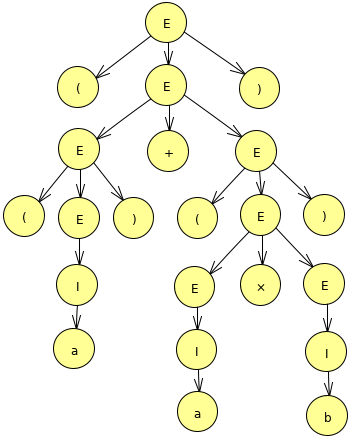
\includegraphics[scale=0.45]{PA07_1b} \end{center}
\subsection{Exercise 2}
\subsubsection{Item a}
G2 is not ambiguous. It however does not represent the same language of G1, something we can prove by considering the string $a \times (a+a)$, which by G1 has a derivation
\begin{alignat*}{6}
	E
	&\xRightarrow[lm]{\ast} E \times E
	&&\xRightarrow[lm]{\ast} I \times E
	&&\xRightarrow[lm]{\ast} a \times E
	&&\xRightarrow[lm]{\ast} a \times (E)
	&&\xRightarrow[lm]{\ast} a \times (E+E) \\
	&\xRightarrow[lm]{\ast} a \times (I+E)
	&&\xRightarrow[lm]{\ast} a \times (a+E)
	&&\xRightarrow[lm]{\ast} a \times (a+I)
	&&\xRightarrow[lm]{\ast} a \times (a+a)
\end{alignat*}
but does not have a derivation by G2, since an expression $E$ can only be extended to the left as an expression, and not to the right.
\subsubsection{Item b}
G3 is not ambiguous. It however does not represent the same language of G1, something we can prove by considering the string $a \times a+a$, which by G1 has a derivation
\begin{alignat*}{6}
	E
	&\xRightarrow[lm]{\ast} E \times E
	&&\xRightarrow[lm]{\ast} I \times E
	&&\xRightarrow[lm]{\ast} a \times E
	&&\xRightarrow[lm]{\ast} a \times E+E \\
	&\xRightarrow[lm]{\ast} a \times I+E
	&&\xRightarrow[lm]{\ast} a \times a+E
	&&\xRightarrow[lm]{\ast} a \times a+I
	&&\xRightarrow[lm]{\ast} a \times a+a
\end{alignat*}
\subsubsection{Item c}
The problem is that G4 describes the string $(a)a$ through the derivation
\begin{alignat*}{7}
	E
	&\xRightarrow[lm]{\ast} J
	&&\xRightarrow[lm]{\ast} I
	&&\xRightarrow[lm]{\ast} Ia
	&&\xRightarrow[lm]{\ast} (E)a
	&&\xRightarrow[lm]{\ast} (J)a
	&&\xRightarrow[lm]{\ast} (I)a
	&&\xRightarrow[lm]{\ast} (a)a
\end{alignat*}
and G1 can not describe this string.
\subsubsection{Item d}
G5 achieves non-ambiguity because it uses new variables to distinguish levels of priority and association rules. Thus, an expression $E$ can only be decomposed into one or a sum of several terms $T$, where each term $T$ can only be decomposed into an identifier $I$, or be promoted again to expression but only if inside parenthesis $(E)$.
}